\documentclass[]{article}
\renewcommand{\baselinestretch}{1.25}

\usepackage[margin=1in]{geometry}
\usepackage{physics}
\usepackage{amsmath, amsfonts, amssymb, amsthm}
\usepackage{amssymb}
\usepackage{graphicx}
\usepackage{hyperref}
\usepackage{empheq}
\usepackage{xcolor}
\usepackage{ulem}

% MATLAB Formatting Code
\usepackage[numbered,framed]{matlab-prettifier}
\lstset{style=Matlab-editor,columns=fullflexible}
\renewcommand{\lstlistingname}{Script}
\newcommand{\scriptname}{\lstlistingname}

% TikZ Things
\usepackage{tikz}
\usetikzlibrary{positioning,shapes}


% Formatting Preferences
\numberwithin{equation}{section}
\usepackage{parskip}
\renewcommand{\figurename}{Fig.}
\allowdisplaybreaks

% Section Heading Settings
\usepackage{enumitem}
\renewcommand{\theenumi}{\alph{enumi}}
\renewcommand*{\thesection}{Problem \arabic{section}}
\renewcommand*{\thesubsection}{\alph{subsection})}
\renewcommand*{\thesubsubsection}{\quad \quad \roman{subsubsection})}

% Math Proof things
\newcommand{\Rel}{\mathcal{R}}
\newcommand{\R}{\mathbb{R}}
\newcommand{\C}{\mathbb{C}}
\newcommand{\N}{\mathbb{N}}
\newcommand{\Z}{\mathbb{Z}}
\newcommand{\Q}{\mathbb{Q}}

\newcommand{\st}{\ : \ }

% Theorem Definition
\newtheorem{definition}{Definition}
\newtheorem{assumption}{Assumption}
\newtheorem{theorem}{Theorem}
\newtheorem{lemma}{Lemma}
\newtheorem{proposition}{Proposition}
\newtheorem{example}{Example}


% Multiagent Robotic Systems Commands
\newcommand{\diam}{\textnormal{diam}}
\newcommand{\radius}{\textnormal{radius}}




%opening
\title{MECH 6V29: Multiagent Robotic Systems- HW 1}
\author{Jonas Wagner}
\date{2022, Febuary 10\textsuperscript{th}}

\begin{document}	

\maketitle

\tableofcontents

%----------------------------------------------------------------------------

% Problem 1 -------------------------------------------------
\newpage
\section{}
% \textbf{Problem:} 
State a summary of first five lectures, preferably by creating a concept map diagram (flow diagram). 
The whole purpose is to make sure that we are clear about the bigger picture, 
and reiterate why are we doing and discussing the specific topics in the class. 
Do not merely write the topics, instead create connections between topics to clarify the flow of information.

\subsection{Big Picture Chart}
\begin{figure}[h]
	\centering
	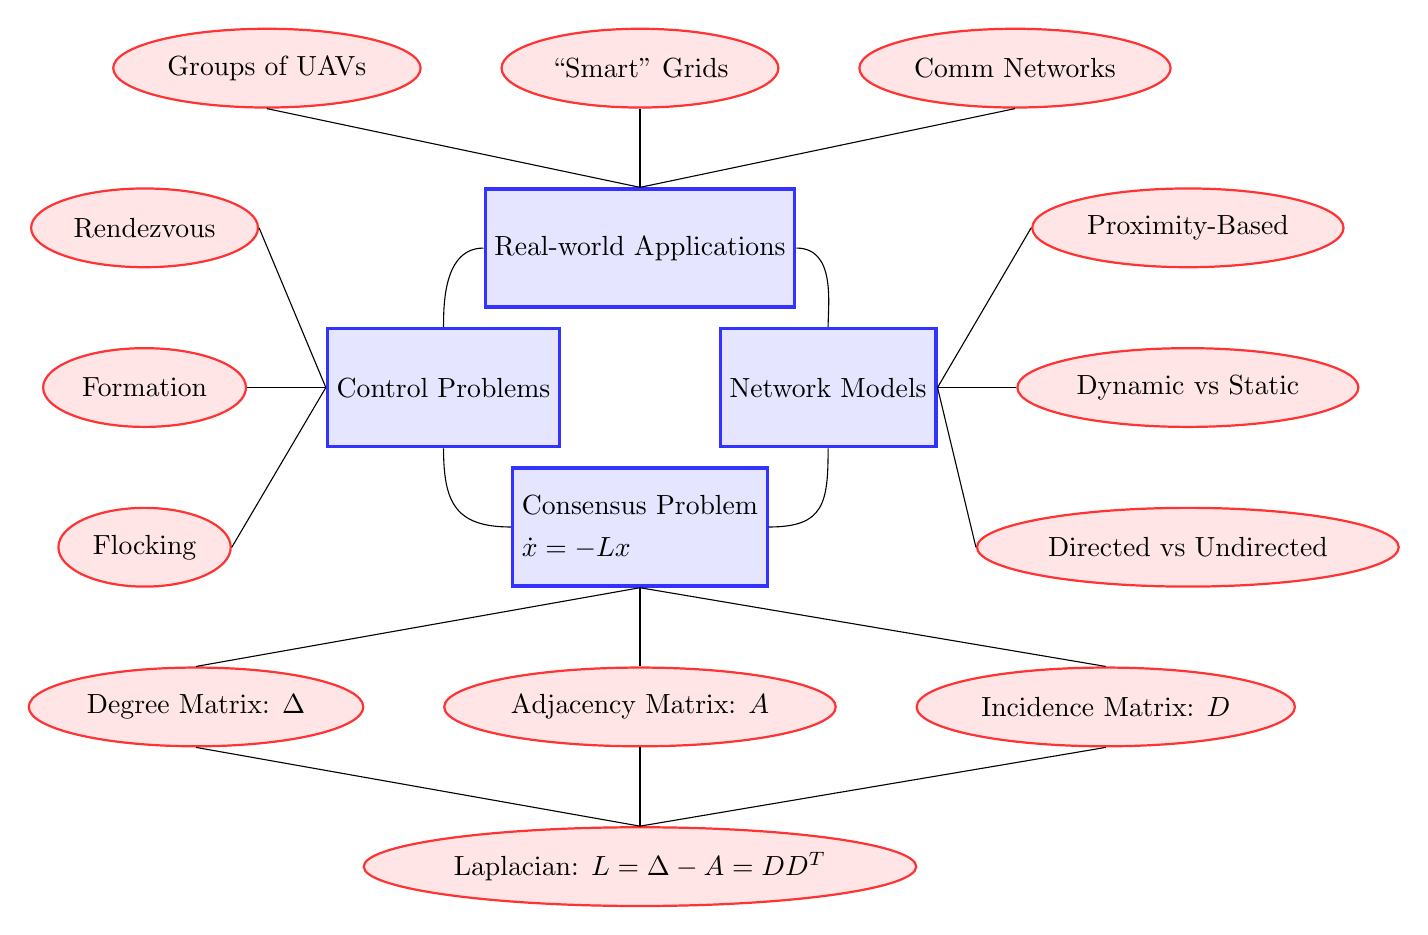
\begin{tikzpicture}[
		empty/.style={coordinate, draw=white!0, fill=white!0, thin, minimum size = 0.1mm},
		block/.style={rectangle, draw=blue!80, fill=blue!10, very thick, minimum size = 15mm},
		extra/.style={ellipse, draw=red!80, fill=red!10, thick, minimum size = 10mm},
		auto,
		% roundnode/.style={circle, draw=green!60, fill=green!5, very thick, minimum size=7mm},
		% squarednode/.style={rectangle, draw=red!60, fill=red!5, very thick, minimum size=5mm},
		]
		%Main Nodes
		\node[empty]	(center)								{};
		\node[block]	(applications)		[above=of center]	{Real-world Applications};
		\node[block]	(ctrl_pblms)		[left=of center] 	{Control Problems};
		\node[block]	(network_model)		[right=of center] 	{Network Models};
		\node[block, text width = 30mm]	(consensus)			[below=of center]	{Consensus Problem $\dot{x}=-L x$};

		%Main Lines
		\draw[-] (applications.west) 	.. controls +(left:5mm) and +(up:3mm)  ..	(ctrl_pblms.north); %controls +(up:5mm) and +(left:5mm)
		\draw[-] (applications.east) 	.. controls +(right:5mm) and +(up:3mm) .. (network_model.north);
		\draw[-] (ctrl_pblms.south) 	.. controls +(down:7mm) and +(left:7mm)  .. (consensus.west);
		\draw[-] (network_model.south)	.. controls +(down:7mm) and +(right:7mm) ..	(consensus.east);

		%Applications
		\node[extra]	(app_2)		[above=of applications]	{``Smart'' Grids};
		\node[extra]	(app_1)		[left=of app_2]			{Groups of UAVs};
		\node[extra]	(app_3)		[right=of app_2]		{Comm Networks};
		\draw[-]	(applications.north) -- (app_1.south);
		\draw[-]	(applications.north) -- (app_2.south);
		\draw[-]	(applications.north) -- (app_3.south);

		%Control Problems
		\node[extra]	(ctr_2)		[left=of ctrl_pblms]	{Formation};
		\node[extra]	(ctr_1)		[above=of ctr_2]		{Rendezvous};
		\node[extra]	(ctr_3)		[below=of ctr_2]		{Flocking};
		\draw[-]	(ctrl_pblms.west)	--	(ctr_1.east);
		\draw[-]	(ctrl_pblms.west)	--	(ctr_2.east);
		\draw[-]	(ctrl_pblms.west)	--	(ctr_3.east);

		%Network Models
		\node[extra]	(graph_2)	[right=of network_model]	{Dynamic vs Static};
		\node[extra]	(graph_1)	[above=of graph_2]			{Proximity-Based};
		\node[extra]	(graph_3)	[below=of graph_2]			{Directed vs Undirected};
		\draw[-]	(network_model.east)	--	(graph_1.west);
		\draw[-]	(network_model.east)	--	(graph_2.west);
		\draw[-]	(network_model.east)	--	(graph_3.west);

		%Consensus

		\node[extra]	(con_2)		[below=of consensus]	{Adjacency Matrix: $A$};
		\node[extra]	(con_1)		[left=of con_2]			{Degree Matrix: $\Delta$};
		\node[extra]	(con_3)		[right=of con_2]		{Incidence Matrix: $D$};
		\node[extra]	(con_4)		[below=of con_2]		{Laplacian: $L = \Delta - A = DD^T$};
		\draw[-]	(consensus.south) 	--	(con_1.north);
		\draw[-]	(consensus.south) 	--	(con_2.north);
		\draw[-]	(consensus.south) 	--	(con_3.north);
		\draw[-]	(con_1.south)		--	(con_4.north);
		\draw[-]	(con_2.south)		--	(con_4.north);
		\draw[-]	(con_3.south)		--	(con_4.north);

	\end{tikzpicture}
	\caption{Diagram of Course Topics (created w/ TikZ)}
	\label{fig:pblm1}
\end{figure}

% Problem 2 -------------------------------------------------
\newpage
\section{}
Go to the following youtube link, and watch a TED talk by Dr. Magnus Egerstedt titled {``Swarm robotics – From local rules to global behaviors''}.
\href{https://www.youtube.com/watch?v=ULKyXnQ9xWA}{https://www.youtube.com/watch?v=ULKyXnQ9xWA}
Then, write down a one paragraph summary, just highlighting the main point or the ‘take-away’ message of the talk. 
Be brief and to the point.

\subsection{Video Summary}
The TED talk by Dr. Magnus Egerstedt title "Swarm Robotics – From local rules to global behaviors" was an introduction to the control of swarm robotic systems and how the field has evolved in the last 10 years.
Swarm robotics algorithms must consist of simple, local, and scalable rules that are safe and reactive for individual agents and result in a predictable emergence.
Much of this is done based on how animals operate within nature and are then particular rules are proven using math.
Currently the consensus problem is fundamental to swarm robotic algorithms and control of the swarm is being done by weighted terms on distances on distances to local agents.
Fundamentally, Swarm Robotics aims to control multi-agent systems with local rules that result in emergence affecting the global behavior of the entire swarm.


% Problem 3 -------------------------------------------------
\newpage
\section{}
In class we saw that an undirected graph G is connected if and only if its Laplacian’s second smallest eigenvalue, $\lambda_2$ is non-zero. 
Using a similar argument as the one in class, show that the number of connected components (i.e. connected subgraphs that are disconnected from each other) is equal to the number of zero eigenvalues of the Laplacian.

\subsection{Definitions}
\begin{definition} \label{def:graph_def}
	\underline{\emph{Graph}} $G(V,E)$ is constructed with \underline{\emph{vertex set}} \[
		V = \qty{v_1,v_2,\dots,v_n}
	\] of $n$ discrete vertices and \emph{\underline{edge set}} \[
		E = \qty{e_1, \dots, e_m} \subseteq V \cross V
	\] consisting of $m$ edges $e_{k=(i,j)} = (v_i,v_j) \forall_{k=1,\dots,m}$ connecting vertices $v_i$ and $v_j$.
\end{definition}

\begin{definition} \label{def:graph_properties}
	Let graph $G(V,E)$ with $V = \qty{v_1,\dots,v_n}$ and $E \subseteq V \cross V$.
	\begin{enumerate}
		\item $G(V,E)$ is considered \underline{\emph{undirected}} if\[
			(v_i,v_j) \in E \iff (v_j,v_i) \in E
		\] otherwise, $G(V,E)$ is considered \emph{directed}.
		\item An undirected graph $G(V,E)$ is considered \underline{\emph{connected}} if there exists a path between any two vertices.
		\item A directed graph $G(V,E)$ is considered \underline{\emph{strongly connected}} if there exists a directed path between any two vertices.
		\item A directed graph $G(V,E)$ is considered \underline{\emph{weakly connected}} if the corresponding undirected graph is connected.
	\end{enumerate}
\end{definition}

\newpage
\begin{definition} \label{def:graph_matrices}
	Let graph $G(V,E)$ with $V = \qty{v_1,\dots,v_n}$ and $E \subseteq V \cross V$.
	\begin{enumerate}
		\item The \underline{\emph{degree matrix}} $\Delta \in \R^{n\cross n}$ is a diagonal matrix defined as \[
			\Delta := \mqty[\dmat{\deg(v_1), \deg(v_2), \ddots, \deg(v_n)}]
		\]
		\item The \emph{\underline{adjacency matrix}} $A \in \R^{n\cross n}$ is a symmetric matrix $(A = A^T)$ defined s.t. \[
			A = [a_{ij}] \st a_{ij} \begin{cases}
				1 &(v_i,v_j) \in V\\
				0 &(v_i,v_j) \notin V
			\end{cases}
		\]
		\item The \emph{\underline{incidence matrix}} $D \in \R^{n \cross m}$ is defined as\[
			D = [d_{ij}] \st d_{ij} \begin{cases}
				1 	&(v_i,-) \in e_{j}\\
				-1	&(-,v_i) \in e_{j}\\
				0	&\text{otherwise}
			\end{cases}
		\]
		\item The \emph{\underline{Laplacian matrix}} $L \in \R^{n \cross n}$ is a symmetric $(L = L^T)$ and strictly semi-positive definite $(L \succeq 0)$ is defined as\[
			L := \Delta - A = D D^T
		\]and\[
			L = \mqty[
				\deg(v_1)	&-a_{12}	&-a_{13}	&\cdots	&-a_{1n}\\
				-a_{21}		&\deg(v_2)	&-a_{23}	&\cdots	&-a_{2n}\\
				\vdots		&\vdots		&\vdots		&\ddots	&\vdots\\
				-a_{n1}		&-a_{n2}	&-a_{n3}	&\cdots	&\deg(v_n)
			]
		\]
		\item For a weighted graph $G(V,E,W)$, the diagonal weighted matrix $W\in \R^{m\cross m}$ is defined as\[
			W = [w_{ij}] \forall_{ij \in E}
		\]
		were $w_{ij}$ are the corresponding weights for $e_{ij} = (v_i,v_j)$.
	\end{enumerate}
\end{definition}

\begin{definition} \label{def:consensus_dynamics}
	Let undirected and unweighted graph $G(V,E)$ with $V = \qty{v_1,\dots,v_n}$ and $E \subseteq V \cross V$.
	The \emph{\underline{consensus dynamics}} of network $G(V,E)$ is defined by\[
		\forall_{i=1,\dots,n} \ \dot{x}_i = \sum_{j\in \mathcal{N}_i} (x_j - x_i)
		\iff \dot{x} = -L x
	\] For the case with weighted graph $G(V,E,W)$ with diagonal weight matrix $W = [w_{ij}]$, 
	\emph{\underline{weighted consensus dynamics}} are given as\[
		\dot{x}_i = \sum_{j\in\mathcal{N}_i} w_{ij} (x_j - x_i) 
		\implies \dot{x} = - L_{w} x
	\]where weighted Laplacian matrix $L_{w}$ is defined as\[
		L_{w} = D W D^T
	\]
\end{definition}

\newpage
\subsection{Preliminary Theorems}
\begin{theorem}\label{thm:L_eig_1_eq_zero}
	Let $G(V,E)$ be an undirected graph.
	The Laplacian matrix $L\in\R^{n \cross n}$ of $G(V,E)$, is symmetric $(L=L^T)$ and positive semi-definite $(L\succeq 0)$.
	Let the eigenvalues of $L$ be\[
		0 \leq \lambda_1 \leq \lambda_2 \leq \cdots \leq \lambda_n
	\] In this undirected case, $L$ will always have eigenvalue $\lambda_1 = 0$ with the corresponding eigenvector of $v_1 = \mathbf{1} = \mqty[1 &1 &\cdots &1]^T$.
	\begin{proof}
		$\lambda_1 = 0$ and $v_1 = \mathbf{1}$ implies\[
			L \mathbf{1} = \lambda_1 \mathbf{1} = 0
		\]Thus
		\begin{align*}
			L \mathbf{1} 
				&= \mqty[
					\deg(v_1)	&-a_{12}	&-a_{13}	&\cdots	&-a_{1n}\\
					-a_{21}		&\deg(v_2)	&-a_{23}	&\cdots	&-a_{2n}\\
					\vdots		&\vdots		&\vdots		&\ddots	&\vdots\\
					-a_{n1}		&-a_{n2}	&-a_{n3}	&\cdots	&\deg(v_n)
				] \mqty[
					1  \\1	\\\vdots	\\1
				] = \mqty[
					\deg(v_1) - \sum_{i\neq 1} a_{1i}\\
					\deg(v_2) - \sum_{i\neq 2} a_{2i}\\
					\vdots\\
					\deg(v_n) - \sum_{i\neq n} a_{ni}\\
				]\\
				&= \mqty[
					\deg(v_1) - \sum_{i\in\mathcal{N}_1} a_{1i}\\
					\deg(v_2) - \sum_{i\in\mathcal{N}_2} a_{2i}\\
					\vdots\\
					\deg(v_n) - \sum_{i\in\mathcal{N}_n} a_{ni}\\
				] = \mqty[
					\deg(v_1) - \deg(v_1)\\
					\deg(v_2) - \deg(v_2)\\
					\vdots\\
					\deg(v_n) - \deg(v_n)\\
				] = \mqty[
					0\\	0\\	\ddots\\ 0
				] = \mathbf{0}
		\end{align*}
		This implies that $\text{span}\qty{1} \subseteq \text{null}\qty(L)$.
	\end{proof}
\end{theorem}

\newpage
\subsection{Solution}
\begin{theorem}\label{thm:k_subgraphs_eq_k_zero_eig}
	Let $G(V,E)$ be an undirected graph.
	The Laplacian matrix $L\in\R^{n \cross n}$ of $G(V,E)$, is symmetric $(L=L^T)$ and positive semi-definite $(L\succeq 0)$.
	Let the eigenvalues of $L$ be\[
		0 \leq \lambda_1 \leq \lambda_2 \leq \cdots \leq \lambda_n
	\]
	Undirected graph $G(V,E)$ will have $k$ connected subgraphs iff $L$ has $k$ zero-valued eigenvalues.
	(i.e) \[
		G(V,E) \text{ contains $k$ connected subgraphs}  
		\iff m_1(\Lambda(L), \lambda_1 = 0) = k
	\]
	\begin{proof}
		The number of block diagonal matrices in the Jordan form of $A$ is equivalent to the number of connected subgraphs, $k$.
		Similarly, if $A$ can be in $k$ blocks then $L$ will also have $k$ blocks.
		In other words,\[
			G(V,E) \text{ contains $k$ connected subgraphs}  
			\iff A \equiv \text{diag}[A_1, A_2, \dots, A_k]
			\iff L \equiv \text{diag}[L_1, L_2, \dots, L_k]
		\] From Theorem \ \ref{thm:L_eig_1_eq_zero}, \[
			\forall_{i=1,\dots,k} \ \Lambda(L_{i}) \ni \lambda_{i,1} = 0
		\] It is also known that the eigenvalues for a block diagonal matrix is composed of all the eigenvalues from the block matrices. 
		(i.e.) \[
			\Lambda(L) = \bigcup_{i=1,\dots,k} \Lambda(L_{i})
		\] with  multiplicities of each similar eigenvalue being summed.
		Since each block, representing a subgraph, has a single zero eigenvalue the multiplicity of $\lambda_1 = 0 \in \Lambda(L)$ is equal to $\sum_{i=1}^{k} 1 = k$. 
		Therefore, \[
			G(V,E) = [G_{i=1,\dots,k}], G_{i} \ \text{connected} 
			\iff m_1(\Lambda(L), \lambda_1 = 0) = k
		\]
	\end{proof}
\end{theorem}

% Problem 4 -------------------------------------------------
\newpage
\section{}
Let the subspace $S$ be\[
	S = \text{span}\qty{\mathbf{1}}^{\perp}
\], i.e.,\[
	x \in S \iff x^T \mathbf{1} = 0
\]
Show that $S$ is $L$-invariant, i.e. $LS \subseteq S$ (i.e. $L x \in S, \forall_{x\in S}$), where $L$ is the Laplacian of an undirected, connected graph.

\subsection{Definitions}
\begin{definition} \label{def:invariant_subspace}
	A subspace $S$ is considered \emph{\underline{invariant}} to matrix $M$ (denoted as $M$-invariant) if\[
		\forall_{x \in S} \ L x \in S
	\]
\end{definition}

\subsection{Solution}
\begin{theorem}\label{thm:pblm4}
	Let subspace $S \subseteq \R^{n}$ be defined as $S = \textnormal{span}\qty{\mathbf{1}}^{\perp}$, (i.e)\[
		x\in S \iff x^T \mathbf{1} = 0
	\] For any $L \in \R^{n\cross n}$ be the Laplacian matrix of an undirected and connected graph, $G(V,E)$, the subspace $S$ is $L$-invariant.
	\begin{proof}
		By Definition \ref{def:invariant_subspace}, $S$ is said to be $L$-invariant if \[
			\forall_{x\in S} \
			 L x \in S
		\] which is equivalent to saying \[
			\forall_{x\in S} \implies (L x)^T \mathbf{1} = 0
		\]
		\begin{align*}
			(Lx)^T \mathbf{1} = 0\\
			x^T L^T \mathbf{1} = 0\\
			\intertext{Since $L$ undirected, $L$ is symetric $L=L^T$,}
			x^T L \mathbf{1} = 0\\
			\intertext{From Theorem \ref{thm:L_eig_1_eq_zero} we have that $\mathbf{1} \in \text{null}\qty(L)$,}
			x^T (0) = 0
		\end{align*}
		Therefore, $\forall_{x\in S} \implies (L x)^T \mathbf{1} = 0$ which by definition proves $S$ is $L$-invariant.
	\end{proof}
\end{theorem}


% Problem 5 -------------------------------------------------
\newpage
\section{}
$K_{1,6}$ is a star graph with one central node and six leaf nodes as shown in \figurename\ref{fig:pblm5}

\begin{figure}[h]
	\centering
	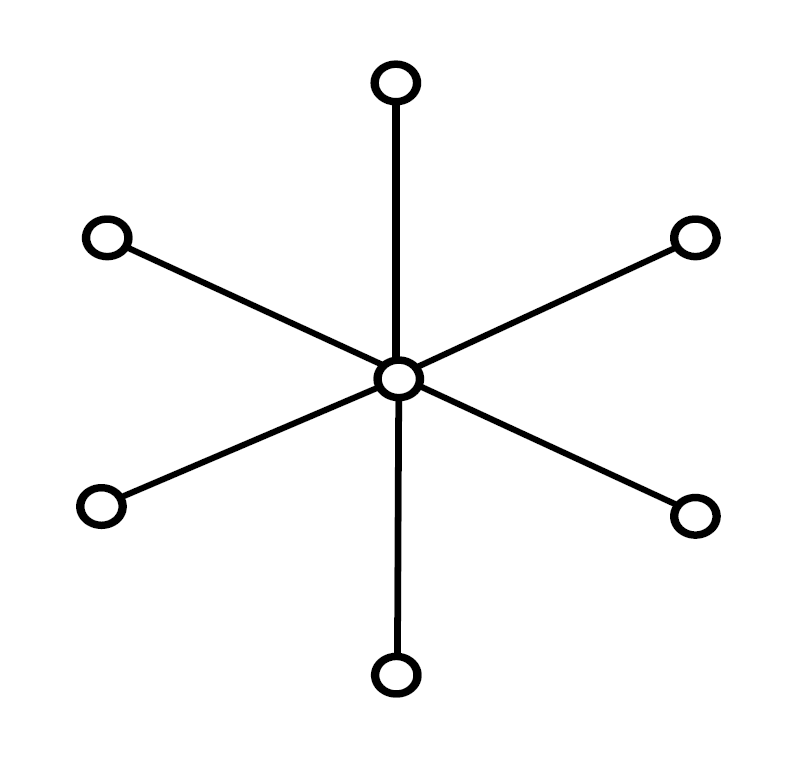
\includegraphics[width=0.2\textwidth]{figs/pblm5.png}
	\caption{Star graph, $K_{1,6}$.}
	\label{fig:pblm5}
\end{figure}

Your task is to show that $K_{1,6}$ can never be an induced subgraph of a $\Delta$-disk proximity graph.

\subsection{Definitions:}
\begin{definition}\label{def:induced_subgraph}
	Let $G(V,E)$ with $V = \qty{v_1,v_2,\dots,v_n}$ 
	and $E = \qty{e_1, \dots, e_m} \subseteq V \cross V$ 
	with $e_k = e_{ij} = (v_i, v_j)$.
	An \emph{\underline{induced subgraph}} of $G(V,E)$ is any $G(V',E')$ with $V'\subset V$ and $E' = [e_{ij}] \ \forall_{v_i, v_j \in V'}$
\end{definition}

\begin{definition}\label{def:Delta-disk_graph}
	Let $V = \qty{v_1,v_2,\dots,v_n}$ be vertices.
	\emph{\underline{$\Delta$-Disk Graphs}} are constructed for a particular $\Delta$ such that \[
		(v_i,v_j) \in E \iff \norm{v_i,v_j} \leq \Delta
	\]
\end{definition}

\subsection{Solution:}
\begin{theorem}
	Let $G(V,E)$ be a $\Delta$-Disk Graph for an arbitrary $\Delta$.
	The star graph $K_{1,6} = G(V_{k16},E_{k16})$ can never be an induced sub graph of $G(V,E)$.
	\begin{proof}
		By Definition \ref{def:Delta-disk_graph}, \[
			E = [e_{ij}] \st e_{ij} = (v_i,v_j) \iff \norm{v_i,v_j} \leq \Delta
		\] Similarly, by Definition \ref{def:induced_subgraph}, an induced subgraph of $G(V,E)$ for vertex set $V' \subset V$ is defined by $G(V',E')$ where $E' = [e_{ij}] \ \forall_{v_i, v_j \in V'}$.
		The associated induced subgraph of $G(V,E)$ for $V' = V_{k16}$ has edges $E' = [e_{ij}] \ st e_{ij} = (v_i,v_j) \iff \norm{v_i,v_j} \leq \Delta$.
		It is clear that for the vertices in $K_{1,6}$, the edges included in $E_{k16}$ is a strict subset of of those within an induced subgraph of those same vertices.
		More simplistically, the edges connecting neighboring leaf nodes that satisfy $\norm{v_i,v_j} \leq \Delta$ would be required for it to be an induced subgraph of a $\Delta$-Disk graph.
	\end{proof}
\end{theorem}

\subsection*{\color{red} Corrected Solution:}
The 'proof' that I used was incomplete. 
I took the baseline geometric assumption that: clearly they would form equilateral triangles so it would be too close for the $\Delta$ of a disk to be the same in all directions because then it would connect with the others.
The actual proof relies on proving this with geometry, essentially:

In order for a $K_{1,6}$ to exist, the center node would have to be connected to 6 nodes that are not also connected.
We look at the angles between such a system and in order for each pair to connect to the center but not each other, the angle between them would have to be greater then $60 \deg$. 
Since there are 6 of these, the angle between them would add up to more then $360 \deg$ and leading to the contradiction.


% Problem 6 -------------------------------------------------
\newpage
\section{}
If $l_{i,j}$ is the shortest path distance (number of edges one needs to follow) between vertices $v_i$ and $v_j$, 
the diameter of the graph is defined as\[
	\diam(G) = \max_{v_i,v_j \in V} l_{i,j}
\] Similarly, if we let $l_{i}^{*}$ (known as the eccentricity of vertex $v_i$) be the longest distance to any vertex from the vertex $v_i$, i.e.,\[
	l_{i}^{*} = \max_{v_j \in V} l_{i,j}
\] then the radius of a graph is defined as\[
	\radius(G) = \min_{v_i \in V} l_{i}^{*}
\] Find the radius and diameter of the following graphs.

\begin{figure}[h]
	\centering
	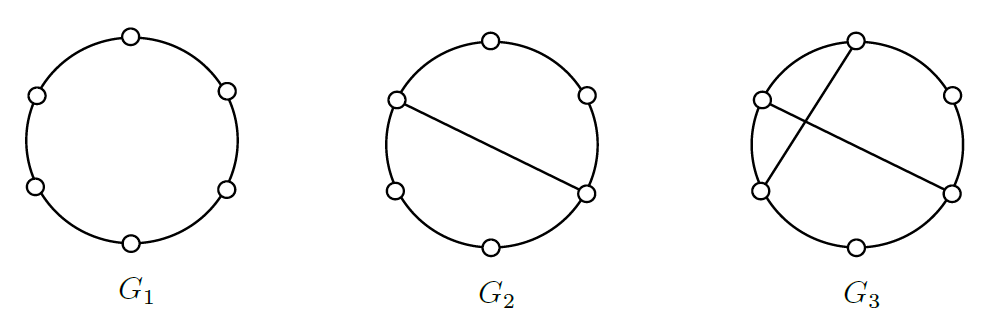
\includegraphics[width=0.7\textwidth]{figs/pblm6.png}
	\caption{Graphs $G_1$, $G_2$, and $G_3$.}
	\label{fig:pblm6}
\end{figure}

\subsection{Definitions:}
\begin{definition}\label{def:path_diam_radius_etc}
	Let $G(V,E)$ be a undirected graph with $V = \qty{v_1,v_2,\dots,v_n}$ 
	and $E = \qty{e_1, \dots, e_m} \subseteq V \cross V$ 
	with $e_k = e_{ij} = (v_i, v_j)$.
	\begin{enumerate}
		\item A \emph{\underline{path}} between two vertices $v_i$ and $v_j$ is a sequence of edges $[e_{i, *}, \dots, e_{*, j}]$ that joins a sequence of vertices $[v_i, \dots, v_j]$.
		\item A \emph{\underline{path length}} is the number of edges in the path. 
		\item The \emph{\underline{shortest path length}} $l_{i,j}$ is the minimum length of all paths between vertices $v_i$ and $v_j$. 
		This quantity is also known as the \emph{\underline{distance}} between $v_i$ and $v_j$, $\text{dist}\qty(v_i,v_j)$.
		\item The \emph{\underline{diameter}} of graph $G(V,E)$ is the maximum distance between any two vertices in the graph. 
		(i.e.)\[
			\diam(G(V,E)) := \max_{v_i,v_j \in V} l_{i,j}
		\]
		\item The \emph{\underline{eccentricity}} of vertex $v_i$, $l_{i}^{*}$, is the largest distance from $v_i$ to any other vertex in the graph. 
		(i.e)\[
			l_{i}^{*} := \max_{v_j \in V} l_{i,j}
		\]
		\item The \emph{\underline{radius}} of graph $G(V,E)$ is the minimum eccentricity of the vertices of the graph.
		(i.e)\[
			\radius(G(V,E)) := \min_{v_i \in V} l_{i}^{*} = \min_{v_i \in V} \max_{v_j \in V} l_{i,j}
		\]
	\end{enumerate}
\end{definition}

\subsection{Solution}
\begin{enumerate}
	\item $G_1$
	\begin{enumerate}
		\item $\diam(G_1) = 3$
		\item $\radius(G_1) = 3$
	\end{enumerate}
	\item $G_2$
	\begin{enumerate}
		\item $\diam(G_2) = \sout{4}{\color{red} 3}$
		\item $\radius(G_2) = 2$
	\end{enumerate}
	\item $G_3$
	\begin{enumerate}
		\item $\diam(G_3) = 2$
		\item $\radius(G_3) = 2$
	\end{enumerate}
\end{enumerate}

% Problem 7 -------------------------------------------------
\newpage
\section{}
Following are some undirected networks on four nodes with the same initial positions.
In which of these networks, nodes converge fastest under the distributed consensus dynamics? 
Explain your answer.

\begin{figure}[h]
	\centering
	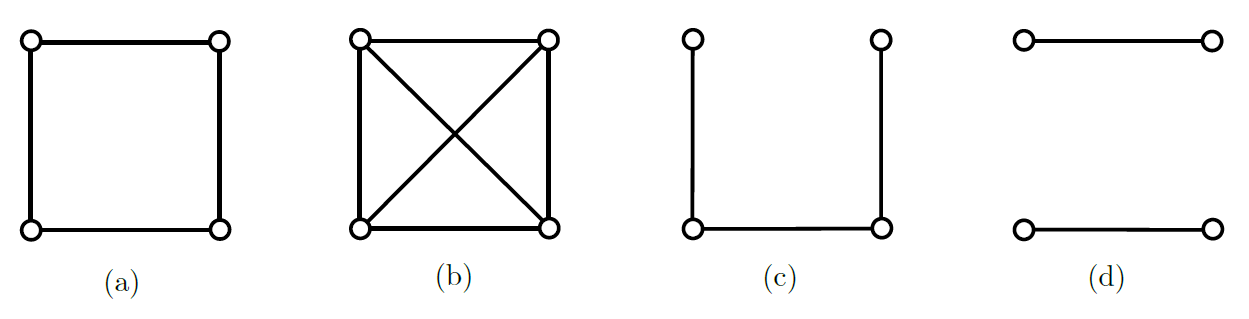
\includegraphics[width=0.7\textwidth]{figs/pblm7.png}
	\caption{Four node undirected networks}
	\label{fig:pblm7}
\end{figure}

\subsection{Network Modeling}
Let vertices $V = \qty{v_1, v_2, v_3, v_4}$ represent each of the 4 nodes in the undirected networks shown in \figurename \ \ref{fig:pblm7}.
Take vertices $v_1, v_2, v_3,$ and $v_4$ as top-left, top-right, bottom-left, and bottom-right respectively.

The edge sets for each network, $\qty{E_a, E_b, E_c, E_d}$, are as follows:
\begin{enumerate}
	\item $E_a = \qty{(v_1,v_2), (v_1, v_3), (v_2,v_4), (v_3,v_4)}$
	\item $E_b = \qty{(v_1,v_2), (v_1, v_3), (v_1,v_4), (v_2,v_3), (v_2,v_4), (v_3,v_4)}$
	\item $E_c = \qty{(v_1, v_3), (v_2,v_4), (v_3,v_4)}$
	\item $E_d = \qty{(v_1,v_2), (v_3,v_4)}$
\end{enumerate}

The Degree $\Delta$, Adjacency $A$, and Laplacian $L$ matrices for each network are laid out in \tablename \ref{tbl:pblm7_matrices}
\begin{table}
	\caption{Network Matrix Representations}
	\[\begin{array}{|c|c|c|c|}
		\hline
			&\Delta &A &L\\
		\hline&&&\\
		G_a	
			&\mqty[\dmat{2,2,2,2}]	
			&\mqty[
				0	&1	&1	&0\\
				1	&0	&0	&1\\
				1	&0	&0	&1\\
				0	&1	&1	&0
			]
			&\mqty[
				2	&-1	&-1	&0\\
				-1	&2	&0	&-1\\
				-1	&0	&2	&-1\\
				0	&-1	&-1	&2
			]\\
		&&&\\\hline&&&\\
		G_b	
			&\mqty[\dmat{3,3,3,3}]	
			&\mqty[
				0	&1	&1	&1\\
				1	&0	&1	&1\\
				1	&1	&0	&1\\
				1	&1	&1	&0
			]
			&\mqty[
				3	&-1	&-1	&-1\\
				-1	&3	&-1	&-1\\
				-1	&-1	&3	&-1\\
				-1	&-1	&-1	&3
			]\\
		&&&\\\hline&&&\\
		G_c
			&\mqty[\dmat{1,1,2,2}]
			&\mqty[
				0	&0	&1	&0\\
				0	&0	&0	&1\\
				1	&0	&0	&1\\
				0	&1	&1	&0
			]
			&\mqty[
				1	&0	&-1	&0\\
				0	&1	&0	&-1\\
				-1	&0	&2	&-1\\
				0	&-1	&-1	&2
			]\\
		&&&\\\hline&&&\\	
		G_d
			&\mqty[\dmat{1,1,1,1}]
			&\mqty[
				0	&1	&0	&0\\
				1	&0	&0	&0\\
				0	&0	&0	&1\\
				0	&0	&1	&0
			]
			&\mqty[
				1	&-1	&0	&0\\
				-1	&1	&0	&0\\
				0	&0	&1	&-1\\
				0	&0	&-1	&1
			]\\
		&&&\\\hline
	\end{array}\]
	\label{tbl:pblm7_matrices}
\end{table}

\subsection{Consensus Dynamics}
From the unweighted consensus dynamics definition in Definition \ref{def:consensus_dynamics}, we have that the continuous time consensus dynamics are governed by the negative Laplacian matrix, $\dot{x} = - L x$.
The eigenvalues of $L$, \[
	\Lambda(L) = \qty{\lambda_1, \lambda_2, \lambda_3, \lambda_4} 
	\st 0 = \lambda_1 \leq \lambda_2 \leq \lambda_3, \leq \lambda_4
\] tell us a lot about the consensus dynamics.
It is known, from Theorem \ \ref{thm:L_eig_1_eq_zero}, that $\lambda_1 = 0$ and this confirms that $\dim(\textnormal{null}\qty(L)) \geq 1$ and that a stead-state consensus is possible.
Further, $\lambda_2$ provides us with a lot of information about how quickly the network will (or will not) converge to a single point.
If $\lambda_2 = 0$, this indicates that the network in not connected and therefore will not converge to a single point due to consensus.
For $\lambda_2 > 0$, the response associated with the slowest mode will converge along the associated eigenvector direction decaying at $e^{-\lambda_2 t}$; 
therefore, as $\lambda_2$ increases the faster the network converges.
Further, this mode will converge to within 2\% of the final location at $t = 4 \lambda_t$.

\newpage
\subsection{Solution}
\textbf{Simple answer:} 
(b) converges fastest, followed by (a), then (c), while (d) converges to two different locations.

\textbf{Justified answer:} 
$\lambda_2$ for each of the networks was calculated as:
\begin{enumerate}
	\item $\lambda_{2}^{(a)} = 2$
	\item $\lambda_{2}^{(b)} = 4$
	\item $\lambda_{2}^{(c)} = 0.585$
	\item $\lambda_{2}^{(d)} = 0$
\end{enumerate}
Clearly, \[
	\lambda_{2}^{(d)} = 0 < \lambda_{2}^{(c)} < \lambda{2}^{(a)} < \lambda_{2}^{(b)}
\] 
$\lambda_{2}^{(d)} = 0$ demonstrates that network (d) is not connected and therefore does not converge.
Additionally, this demonstrates that the fastest to slowest convergence is (b), (a), then (c).

% Problem 8 -------------------------------------------------
% \newpage
\section{}
What is the necessary and sufficient condition for the consensus to happen in the case of static directed networks? 
Derive this condition.

\subsection{Solution}
This question isn't very specific about what types of conditions are being referred to, so one of the many equivalent conditions that are both necessary and sufficient is that the the positive semi-definite, yet not generally symmetric, directed Laplacian matrix \[
	L = \Delta^{in} - A^{in}
\] that describes the dynamics of the directed network in consensus as\[
	\dot{x} = - L x
\]\textbf{ has only one zero-valued eigenvalue, $\lambda_1 = 0$, that is associated with eigenvector $\mathbf{1}$}.
This also is equivalent to saying that the null-space of $L$ is strictly defined as:\[
	\textnormal{null}\qty(L) = \textnormal{span}\qty{\mathbf{1}}
\] The proof of these conditions is simple:

Consensus occurs when\[
	\lim_{t \to \infty} x = x_f \st x_f \in \textnormal{span}\qty{\mathbf{1}}
\] which is equivalent to saying \[
	\textnormal{null}\qty(L) = \textnormal{span}\qty{\mathbf{1}} 
	\land L \succeq 0
\]

As a linear system $\dot{x} = -L x$ only requires the given $L \succeq 0$ to be considered marginally stable; however explicitly specifying that the associated eigenvector with $\lambda_1 = 0$ is $\mathbf{1}$ is also necessary to ensure that all final states are equivalent.

\newpage
\appendix
\section{MATLAB Code:}\label{apx:matlab}
All code I write in this course can be found on my GitHub repository:\\
\href{https://github.com/jonaswagner2826/MECH6V29_MultiagentRoboticSystems}{https://github.com/jonaswagner2826/MECH6V29\_MultiagentRoboticSystems}

\bibliographystyle{ieeetran}
\bibliography{refs.bib}
\cite{*}

\end{document}
